\documentclass{article}
\usepackage{latexsym,amsmath,xcolor,multicol,booktabs,calligra}
\usepackage{ctex,hyperref,graphicx,pstricks,listings,stackengine,tikz,listings}
\usetikzlibrary{angles}
\usetikzlibrary{quotes}
\usetikzlibrary{shapes.geometric}
\definecolor{primaryD}{HTML}{00695C}
\begin{document}

\begin{tikzpicture}
\node[below,left]at(0,0){$O$};
\draw[->] (0,0) -- (3.5,0) node[right] {$x$};
\draw[->] (0,0) -- (0,2.5) node[above] {$y$};
\draw (0,2)--(3,2)--(3,0);
\draw[dashed](1.5,-0.3)--(1.5,2.3);
\draw[dashed](-0.3,1)--(3.3,1);
\node[below]at(3,0){$g_x$};
\node[left]at(0,2){$g_y$};
\node (comment) [scale=0.8] at (2.5,-0.7,0) {靠近原点的子区域};
\draw [->] (comment) to [in = 270, out = 180] (0.75,0.3);
\foreach \x in {0.2,0.4,...,2.8}
\foreach \y in {0.2,0.4,...,1.8}
\node at(\x,\y){.};
\end{tikzpicture}
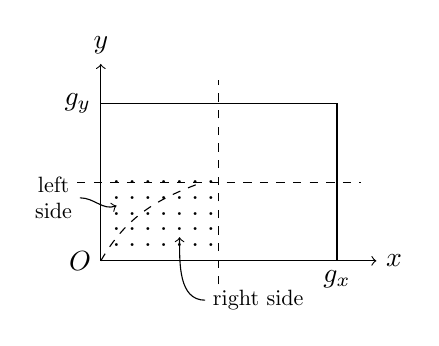
\begin{tikzpicture}
\node[below,left]at(0,0){$O$};
\draw[->] (0,0) -- (3.5,0) node[right] {$x$};
\draw[->] (0,0) -- (0,2.5) node[above] {$y$};
\draw (0,2)--(3,2)--(3,0);
\draw[dashed](1.5,-0.3)--(1.5,2.3);
\draw[dashed](-0.3,1)--(3.3,1);
\node[below]at(3,0){$g_x$};
\node[left]at(0,2){$g_y$};
\draw [dashed](0,0)to[in=200,out=60](1.3,1);
\node (comment1) [scale=0.8,align=center] at (-0.6,0.8) {left\\side};
\draw [->] (comment1) to [in = 200, out = 0] (0.2,0.7);
\node (comment2) [scale=0.8] at (2,-0.5,0) {right side};
\draw [->] (comment2) to [in = 270, out = 180] (1,0.3);
\foreach \x in {0.2,0.4,...,1.4}
\foreach \y in {0.2,0.4,...,1}
\node at(\x,\y){.};
\end{tikzpicture}

\end{document}